OpenQuake-risk has been developed by the scientific members of the GEM Model Facility, following an extensive review of existing software to calculate seismic risk (\citep{CrowleyH.2010} ). 
%
% ------------------------------------------------------------------------------
\section{OpenQuake-risk: main concepts}
OpenQuake-risk is coded in the Python programming language and is currently linked to OpenQuake-hazard, but there are plans to allow users to input their own hazard in the future. The procedure to calculate risk outputs is currently as follows:
\begin{enumerate}

\item Read the hazard input file, the vulnerability model input file, the exposure model input file and the calculation settings.

\item Combine the ground motions from OpenQuake-hazard (either from hazard curves or ground motion fields depending on the calculation workflow) with the vulnerability for each asset defined in the exposure model, to calculate the losses to the assets.

\item Post-process the losses in an appropriate manner to produce loss curves, maps and statistics. 

\end{enumerate}
%
% ------------------------------------------------------------------------------
\section{Calculation Workflows}
OpenQuake currently comprises three risk calculation workflows: one computing losses due to a single event, and the other two computing seismic risk due to most or all of the possible events that might occur in a given region within a certain time span. The calculation workflows are comprised of a number of separate calculators. In order to run any of the calculation workflows, it is necessary to define the geographic coordinates of the region of interest, the type of calculations, the path to the input files (vulnerability and exposure models), the type of results that are to be produced and several parameters necessary for the hazard calculations. Currently, a configuration file to be provided to OpenQuake incorporates this information.

The following three calculation workflows are thus supported:
\begin{itemize}
\item \textbf{Deterministic Event-Based Risk}: this calculation sequence is capable of computing losses and loss statistics due to a single,
deterministic earthquake, for a collection of assets (see Figure \ref{fig:Scheme_detrisk_calc}). Such analyses are of importance, for example, for emergency management planning and for raising societal awareness of risk. 

\begin{figure}[ht]
\centering
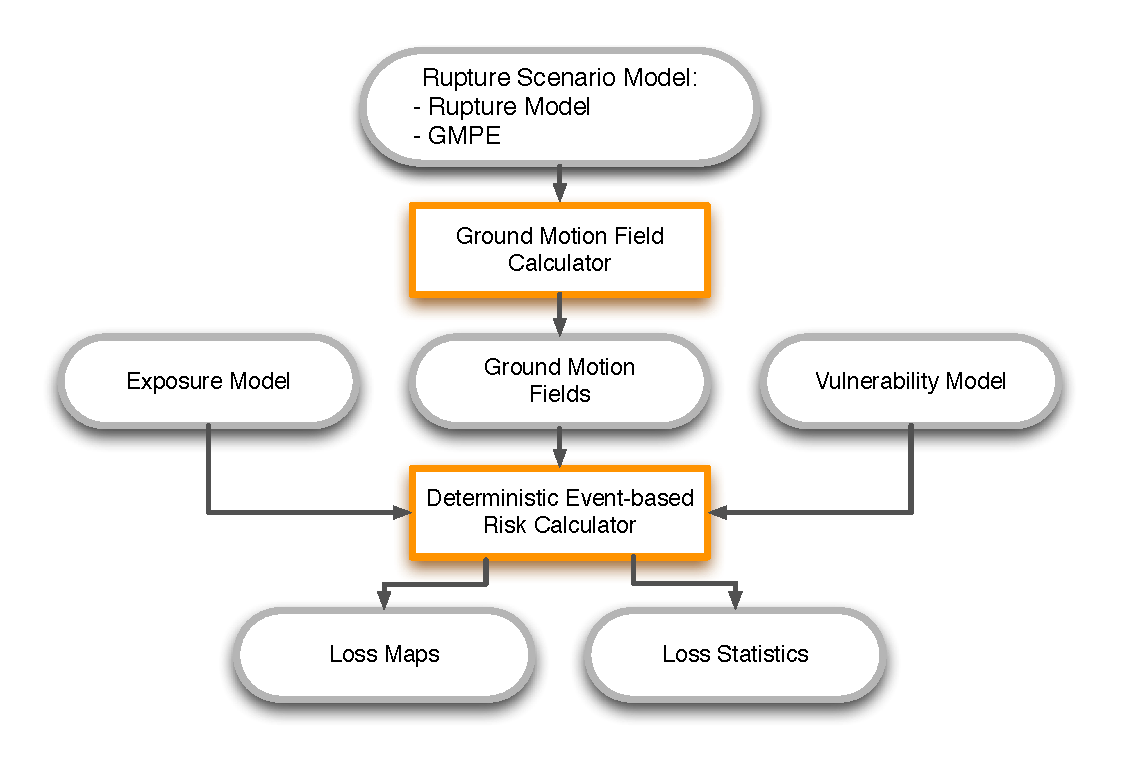
\includegraphics[width=10cm,height=8cm]{./Figures/Part_Risk/Scheme_Deter_calc.eps}
\caption{Workflow of the deterministic event-based risk calculations.}
\label{fig:Scheme_detrisk_calc}
\end{figure}

\item \textbf{Probabilistic Event-Based Risk}: this calculation workflow computes the probability of losses and loss statistics for a collection of
assets, based on the probabilistic hazard (see Figure \ref{fig:Scheme_probrisk_calc}). The losses are calculated with an event-based approach, such that the simultaneous losses to a set of assets can be calculated.

\begin{figure}[ht]
\centering
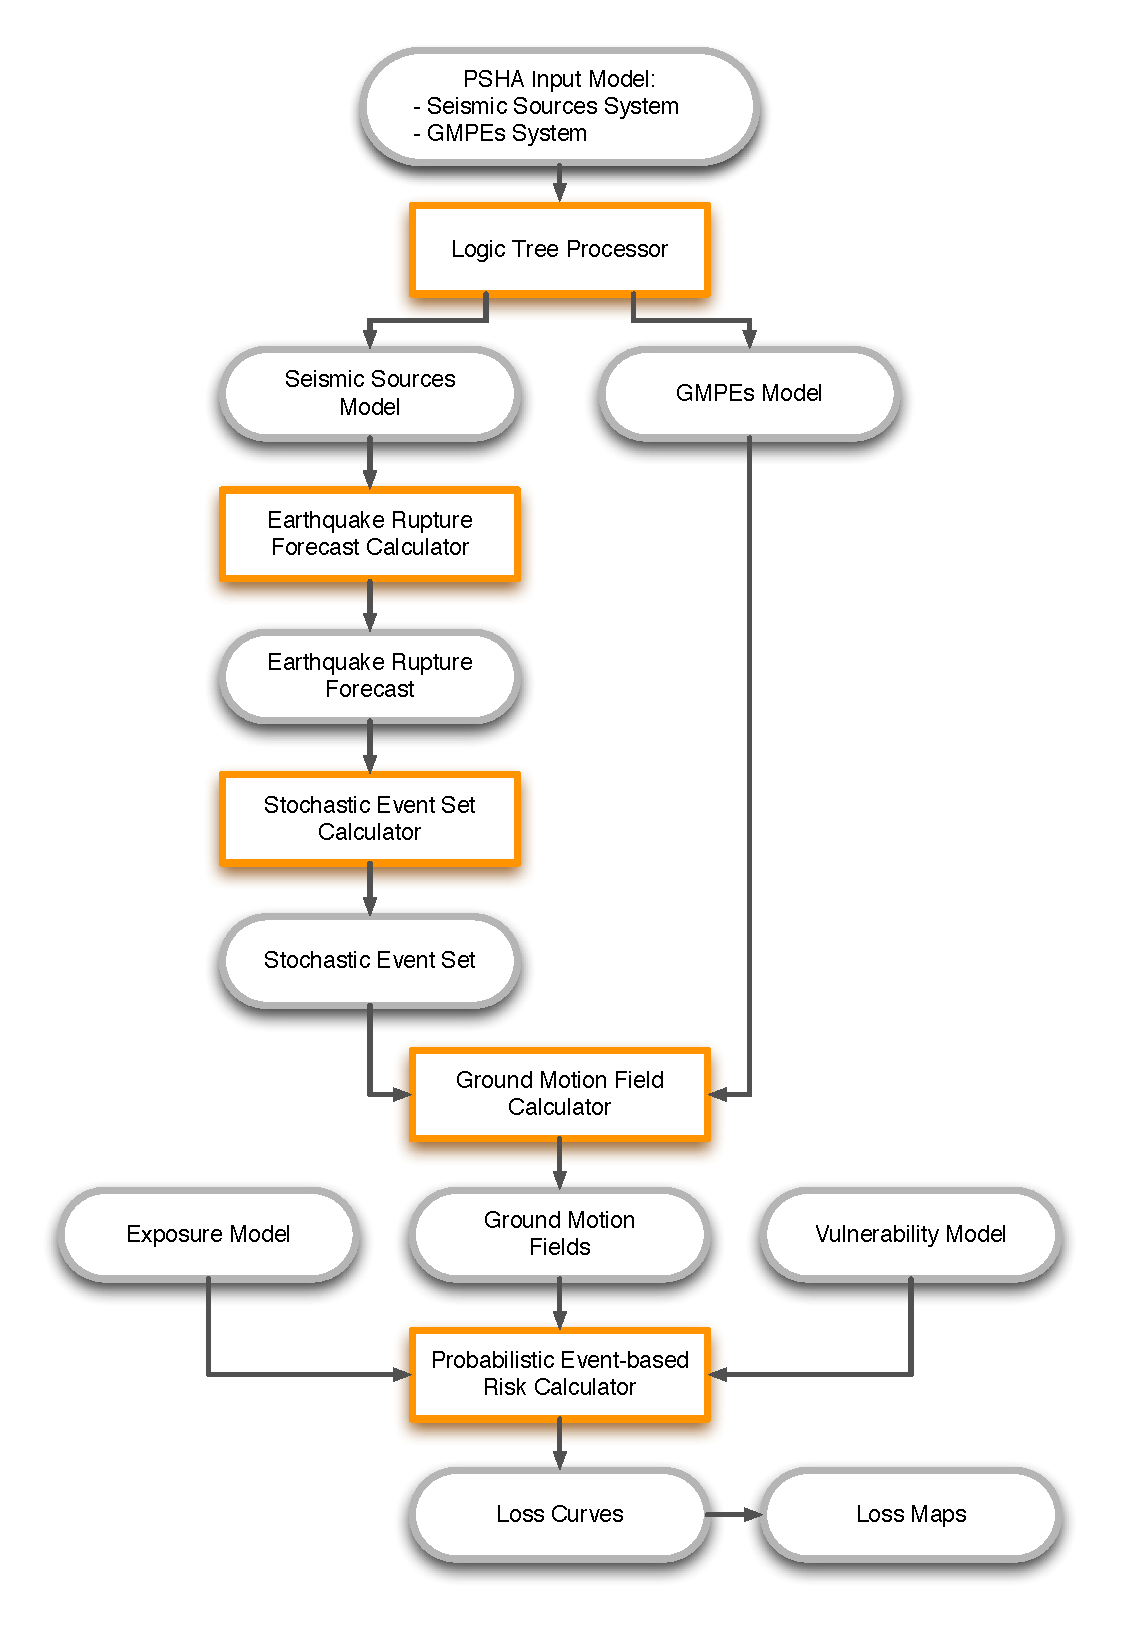
\includegraphics[width=10cm,height=17cm]{./Figures/Part_Risk/Scheme_Prob_calc.eps}
\caption{Workflow of the probabilistic event-based risk calculations.}
\label{fig:Scheme_probrisk_calc}
\end{figure}

\item \textbf{Classical PSHA-Based Risk}: this calculation workflow leads to the computation of the probability of losses and loss statistics for
single assets, based on the probabilistic hazard (see Figure \ref{fig:Scheme_classrisk_calc}). The output of this calculator is useful for comparative risk assessment between assets at different locations.
\end{itemize}

\begin{figure}[ht]
\centering
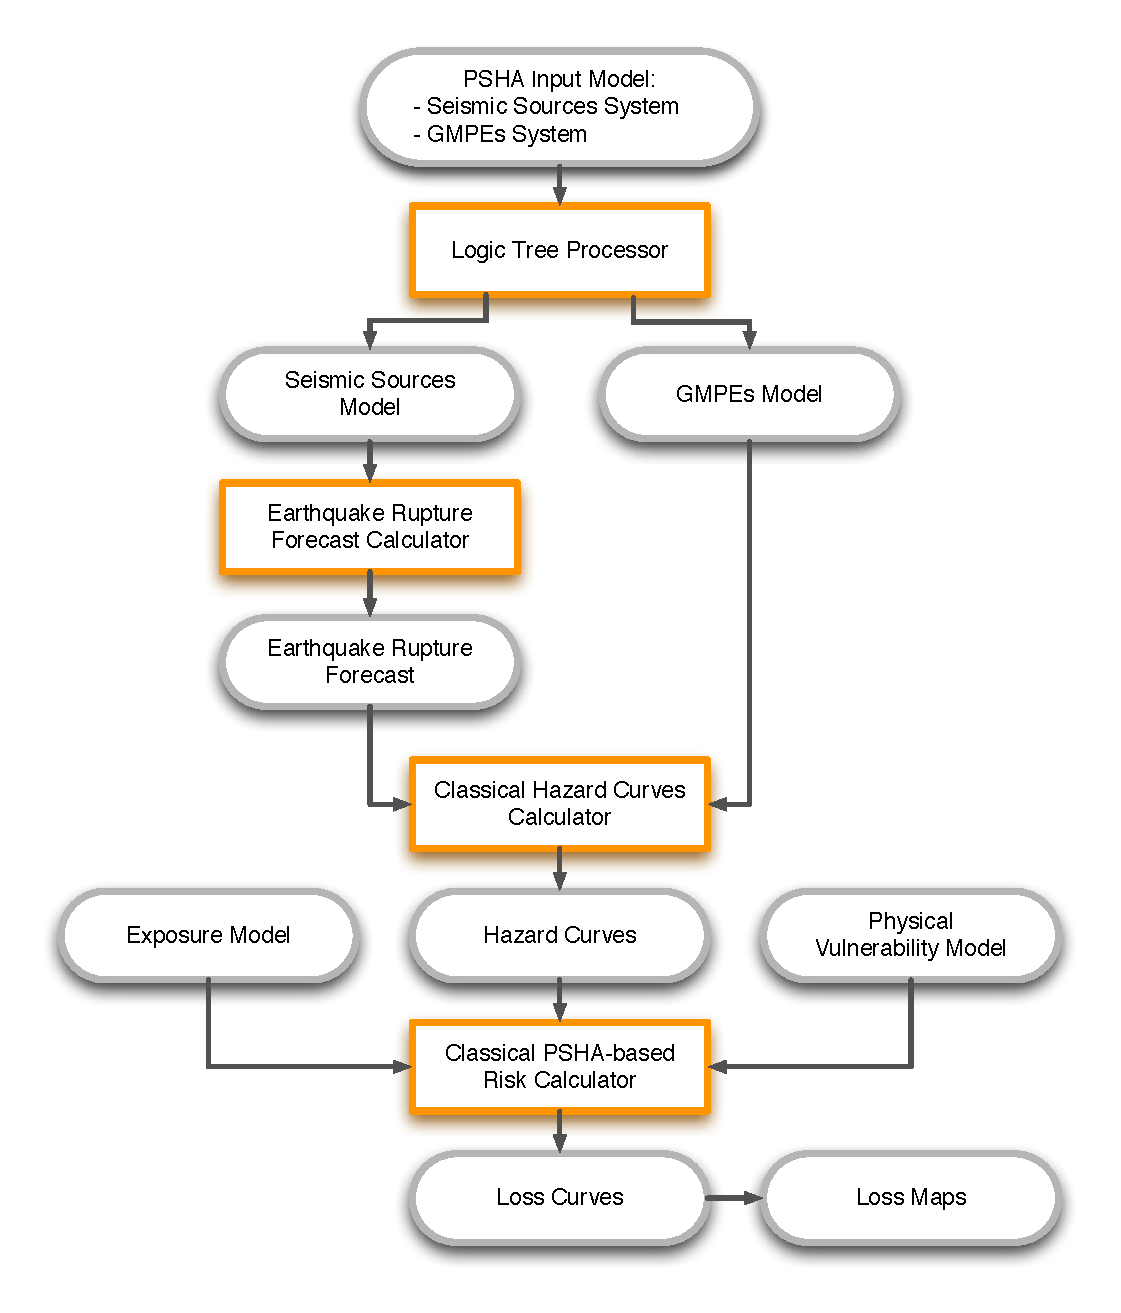
\includegraphics[width=10cm,height=13cm]{./Figures/Part_Risk/Scheme_PSHA_calc.eps}
\caption{Workflow of the classical PSHA-based risk calculations.}
\label{fig:Scheme_classrisk_calc}
\end{figure}

The hazard calculators in the aforementioned workflows have already been described in the hazard section of this book, and so the following chapters focus on the input, the calculators required for the three distinct workflows (deterministic event-based risk calculator, probabilistic event-based risk calculator and classical PSHA-based risk calculator) and their output.
%